
\documentclass[crop,tikz]{standalone}
\usepackage[utf8]{inputenc}
\usepackage{tikz}
\usepackage{pgfplots}
\pgfplotsset{compat=newest}
\usepgfplotslibrary{groupplots}
\begin{document}
% This file was created by matplotlib2tikz v0.6.15.
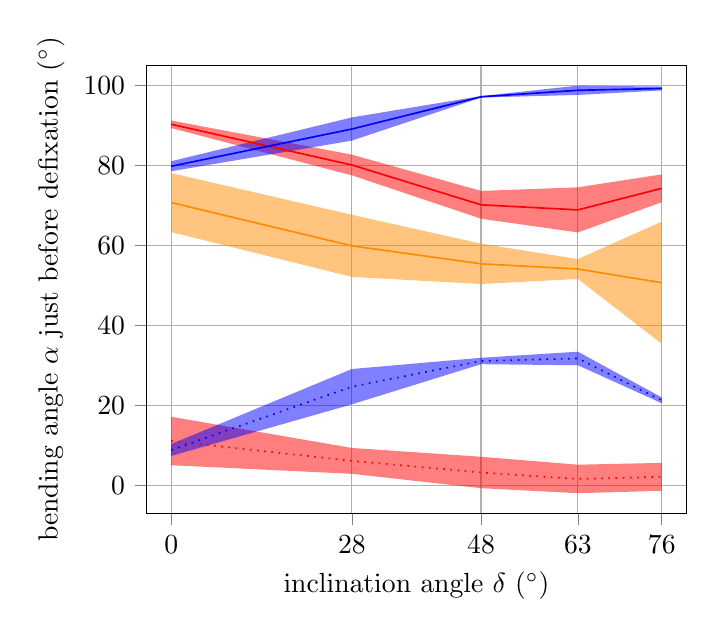
\begin{tikzpicture}

\definecolor{color0}{rgb}{1,0.549019607843137,0}

\begin{axis}[
xlabel={inclination angle $\delta$ ($^\circ$)},
ylabel={bending angle $\alpha$ just before defixation ($^\circ$)},
xmin=-3.8, xmax=79.8,
ymin=-7.04601616234104, ymax=105.002397477296,
tick align=outside,
tick pos=left,
xmajorgrids,
x grid style={lightgray!92.026143790849673!black},
ymajorgrids,
y grid style={lightgray!92.026143790849673!black},
xtick={0, 28, 48, 63, 76}
]
\path [fill=red, fill opacity=0.5] (axis cs:0,89.3108632973758)
--(axis cs:0,91.1927386978303)
--(axis cs:28,82.6652475798688)
--(axis cs:48,73.590706359172)
--(axis cs:63,74.4926463070287)
--(axis cs:76,77.7293311927181)
--(axis cs:76,70.7702020202057)
--(axis cs:76,70.7702020202057)
--(axis cs:63,63.2191122216144)
--(axis cs:48,66.6566833851307)
--(axis cs:28,77.4839519694055)
--(axis cs:0,89.3108632973758)
--cycle;

\path [fill=color0, fill opacity=0.5] (axis cs:0,63.3103456358201)
--(axis cs:0,78.0535829182683)
--(axis cs:28,67.6261190268708)
--(axis cs:48,60.404904003335)
--(axis cs:63,56.5646825244646)
--(axis cs:76,65.9290909090922)
--(axis cs:76,35.3795370989456)
--(axis cs:76,35.3795370989456)
--(axis cs:63,51.5925521780842)
--(axis cs:48,50.3384078458527)
--(axis cs:28,52.0967315962388)
--(axis cs:0,63.3103456358201)
--cycle;

\path [fill=blue, fill opacity=0.5] (axis cs:0,78.5125314409266)
--(axis cs:0,81.0149261206704)
--(axis cs:28,91.9683456116381)
--(axis cs:48,97.3074524078078)
--(axis cs:63,99.9092877664037)
--(axis cs:76,99.6825757575801)
--(axis cs:76,98.7198529411921)
--(axis cs:76,98.7198529411921)
--(axis cs:63,97.5828838531418)
--(axis cs:48,96.9360565935972)
--(axis cs:28,86.1721751564633)
--(axis cs:0,78.5125314409266)
--cycle;

\path [fill=red, fill opacity=0.5] (axis cs:0,5.04723465211582)
--(axis cs:0,17.1463232819709)
--(axis cs:28,9.35963934053291)
--(axis cs:48,7.15504469824248)
--(axis cs:63,5.17474298343682)
--(axis cs:76,5.62287878787649)
--(axis cs:76,-1.34634163324682)
--(axis cs:76,-1.34634163324682)
--(axis cs:63,-1.95290645144843)
--(axis cs:48,-0.699023271782201)
--(axis cs:28,2.88973653562711)
--(axis cs:0,5.04723465211582)
--cycle;

\path [fill=blue, fill opacity=0.5] (axis cs:0,7.36982379358714)
--(axis cs:0,10.3349812347311)
--(axis cs:28,29.0883738290973)
--(axis cs:48,31.8928570056969)
--(axis cs:63,33.4107364473781)
--(axis cs:76,21.99356060606)
--(axis cs:76,20.5284090908999)
--(axis cs:76,20.5284090908999)
--(axis cs:63,30.030461545651)
--(axis cs:48,30.2910959582937)
--(axis cs:28,20.2633694417523)
--(axis cs:0,7.36982379358714)
--cycle;

\addplot [semithick, red, forget plot]
table {%
0 90.2518009976031
28 80.0745997746371
48 70.1236948721513
63 68.8558792643215
76 74.2497666064619
};
\addplot [semithick, color0, forget plot]
table {%
0 70.6819642770442
28 59.8614253115548
48 55.3716559245939
63 54.0786173512744
76 50.6543140040189
};
\addplot [semithick, blue, forget plot]
table {%
0 79.7637287807985
28 89.0702603840507
48 97.1217545007025
63 98.7460858097728
76 99.2012143493861
};
\addplot [semithick, red, dotted, forget plot]
table {%
0 11.0967789670434
28 6.12468793808001
48 3.22801071323014
63 1.61091826599419
76 2.13826857731484
};
\addplot [semithick, blue, dotted, forget plot]
table {%
0 8.85240251415913
28 24.6758716354248
48 31.0919764819953
63 31.7205989965146
76 21.26098484848
};
\end{axis}

\end{tikzpicture}
%% End matplotlib2tikz content %% 
\end{document}